
% Put **your** name and the proper due date in place

% Copy the lstlisting and figure code as many times as you need
% Be sure to put in your own file names if appropriate

% Note that the \epsfig commands are currently commented out - until the
% files exist, processing this code without them will result in an error
% so leave the comments until you have created the graphics files!

\documentclass{article}
\usepackage{amsmath}    % loads AMS-Math package
\usepackage{epsfig}     % allows PostScript files
\usepackage{listings}   % allows lstlisting environment
\usepackage{moreverb}   % allows listinginput environment
\usepackage{vmargin}    % allows better margins
\usepackage{epstopdf}   % converts eps to pdf
\usepackage{enumerate}  % allows the use of alphabetical lists
\usepackage{graphicx}   % allows the use of image files
\usepackage{wrapfig}    % wraps the figures
\usepackage{lscape}     % allows the use of landscape moder
\usepackage{rotating}   % rotates the image
\setpapersize{USletter} % sets the paper size
\setmarginsrb{1in}{0.1in}{1in}{0.2in}{12pt}{11mm}{0pt}{11mm} %sets margins 
\providecommand{\e}[1]{\ensuremath{\times 10^{#1}}}
\begin{document}
\begin{center}
\rule{6.5in}{0.5mm}
{\bf \large ECE 350 -- Spring 2016}\\~\\
{\bf \huge HW 2 - Register File}\\~\\
Sivaneshwaran Loganathan\\
Lab Section 07, February 11, 2016\\
\rule{6.5in}{0.5mm}
\end{center}
\section{Design Implementation}
To build a register file, multiple submodules needed to be implemented or obtained from the Altera library. The submodules are shown below
\begin{enumerate}
	\item Altera Library
	\begin{enumerate}
		\item DFFE - D Flip Flop with Enable bit
	\end{enumerate}
	\item Personal Created Modules
	  \begin{enumerate}
	  	\item 5 to 32 Decoder
	  	\item Register
	  	\item Tri State Buffer
	  \end{enumerate}
\end{enumerate}
The register used a generator loop to generate the 32 DFFE inside it so that it would be able to store all 32 bits. The output of each register is then connected to a Tri State Buffer where a 5 to 32 decoder was used to select the register to read from. In the case of write, a 5 to 32 decoder was used to determine which register to write too. Each bit from the output of the decoder was an input to an AND gate alongside with the ctrl writeEnable signal. This was then connected to each of the register in the generator loop.
\section{Timing Waveform}
To determine the timing waveform, I fixed the clock cycle. I then did a write operation to  clock cycle. I then did a read in the next clock cycle. If there were any glitches as seen by the very small diamond shapes in the output waveform, it represents a distorted wave. In this case, this represents a clock frequency where the register file can't function. If the waveform looks fine, the clock frequency was increased.


\begin{figure}[ht!]
\begin{center}
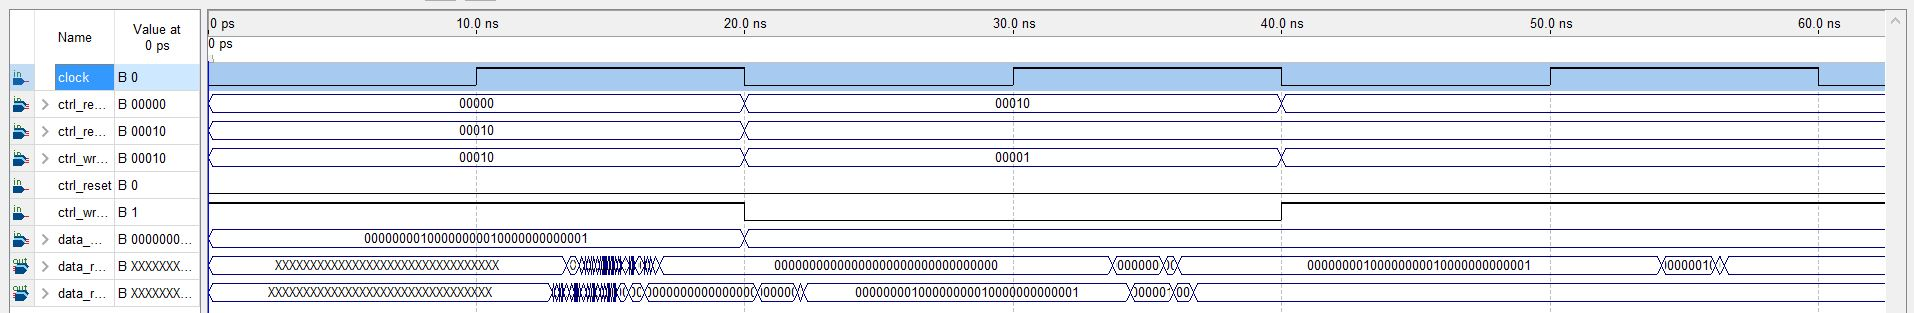
\includegraphics[scale=0.4]{timingSim.JPG}
\caption{Waveform Vector for Clock Rate = 50MHz}
\end{center}
\end{figure}


\end{document}


